\section*{Problema 14.57, Z}

\noindent Cada uno de los dos péndulos que se ilustran en la figura consiste en una esfera sólida uniforme de masa $M$ sostenida por una varilla de masa despreciable; no obstante, la esfera del péndulo $A$ es muy pequeña, en tanto qeu la esfera del péndulo $B$ es mucho más grande. Obtenga el periodo de cada péndulo para desplazamientos cortos. ¿Qué esfera tarda más en completar una oscilación?



\begin{figure}[H]
	\centering
	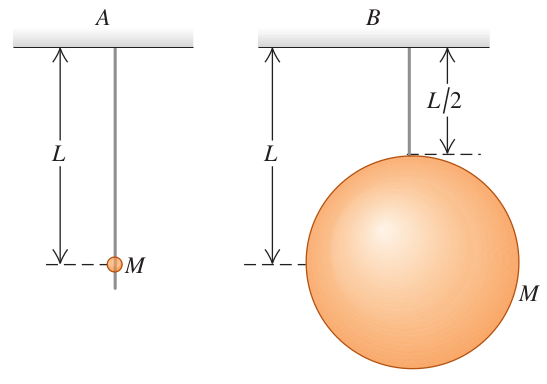
\includegraphics[scale=0.4]{./img/t8.png}
\end{figure}







%%%%